\title{\bf Atmospheric effects}

\section{Basics \& Nomenclature}

Ground-based astronomers must reckon with the effect of the atmosphere
on their observations. The atmosphere imprints wavelength-dependent
absorption on the incoming light. It glows with a complex,
time-dependent and space-dependent spectrum.  It refracts the light as
a function of zenith angle and wavelength. Finally, turbulence in the
atmosphere distorts the incoming light's wave fronts, leading to image
motion and blur.

When calculating the effects of the atmosphere, the zenith angle $z$
is a critical factor. In the plane-parallel approximation, which
virtually always holds, the column density of atmosphere at $z$ scales
as the {\it airmass}, $a = 1 / \cos z$. 

Figure \ref{fig:absorption} shows the atmospheric transmission at
zenith $t(z=0^\circ)$ as a function of wavelength at sea level. The
transmission at other airmasses is:
\begin{equation}
t(z) = [t(z=0^\circ)]^a,
\end{equation}
where $a$ is the airmass. It also depends on height above sea level.
The sharp absorption features are known as {\it telluric lines}; the
strongest of these are the Fraunhofer A and B bands around
7000--7500 \AA, due to O$_2$.

The ultraviolet and higher energy photons are essentially entirely
absorbed below $3500$ $\AA$, mostly due to ozone. Starting in the
near-infrared and continuing to about mm wavelengths, the atmosphere
has strong absorption bands associated with water vapor and carbon
dioxide.  The exact level of absorption depends on the humidity,
pressure, and temperature.  This means the transmission spectra
depends on time and the average conditions vary considerably between
different locations. Favorable locations include but are not limited
to the high deserts of Chile and the South Pole.

Figure \ref{fig:emission} shows the atmospheric emission as a function
of wavelength. The components of this emission include a scattered
light component. This scattered light comes primarily from ground
sources and the Moon. When the Moon is out it tends to dominate the
continuum regions of the sky spectra; this spectrum then resembles the
solar spectrum. Other scattered light yields a spectrum that reflects
the light source, often from mercury or sodium lines due to artificial
lighting (with the sodium lines occasionally containing a broad
component due to high pressure sodium lamps; \citealt{osterbrock76a}).
The scattered light emission is dependent on Moon phase and angle to
the Moon (or to other sources) and is fairly smoothly varying in time
and angle.

Emission also originates from the atmosphere itself.  In the optical
and near-infrared, this emission is dominated by fluorescence due to
excitation of atoms and molecules, known as {\it airglow}. Neutral
oxygen has several important lines, and OH exhibits a suite of
rotation-vibrational modes (\citealt{osterbrock96a,
osterbrock97a}). The airglow varies rapidly in time (over tens of
minutes) and in angle (on scales of tens of arcminutes). Past 2--3
microns, the spectrum starts to be dominated by thermal emission
(though at these wavelengths the telescope itself becomes the more
important background).

An important source of background emission is also the {\it zodiacal
light}, which originates in the Solar System and concentrated to the
ecliptic plane, with a complex dependence on angle.

The light that is transmitted from outside the atmosphere to the
telescope is also refracted by the atmosphere. At reasonable zenith
angles and almost all conditions, the atmosphere can be treated as
plane parallel, and all that matters for the refraction effects is the
index of refraction at the telescope. This index depends primarily on
pressure (and thus altitude) and to a lesser extent on temperature and
relative humidity. Snell's Law is a strong enough function of zenith
angle that for fields of view above a few arcminutes, usually one
needs to worry about differential refraction across the field inducing
both a monopole and a quadrupole distortion.

Because the index of refraction is a function of wavelength, the
refraction means that the images of different wavelengths will appear
in different locations. In this way, the atmosphere acts as a weak
prism, dispersing the light along the direction to and from zenith,
called the {\it parallactic angle}. This effect can be up to a couple
of arcseconds and so be very significant.

Finally, the light being transmitted usually arrives at the atmosphere
from infinity in plane waves, except in the case of radio waves which
experience interstellar scintillation. These plane waves are distorted
when passing through the atmosphere. These distortions occur because
of turbulent mixing between atmospheric layers with different indices
of refraction, which cause fluctuations in the wave fronts. These
distortions are known generically as {\it seeing}.

Under good conditions, the seeing is dominated by a turbulent surface
layer near the telescope and a handful of thin turbulent layers within
a few kilometers of the surface. The index of refraction varies over
short length scales in these turbulent layers. The variation of this
index leads the electromagnetic plane waves to become wrinkled in a
time-dependent fashion. The coherence length of the waves $r_0$
depends on conditions, but under reasonably good conditions is about
20~cm and because of the variation of the index of refraction with
wavelength scales as $\lambda^{6/5}$.

This coherence length sets the diffraction limit for ground-based
telescopes. This means that optical observations are typically limited
to $\sim$ 1 arcsec FWHM resolution, and that telescopes above a
diameter of about 20 cm do not continue to benefit from better
diffraction limits.

Because the distortion of the wavefronts on larger scales than the
telescope diameter varies over time, it contributes to image motion
over time; that is, the diffraction limited spot changes location. For
long enough exposures this effect will also contribute to the
effective resolution of the image. This effect is more severe the
smaller the telescope.

The shape of the atmospheric point spread function within a few times
the FWHM can be predicted from a study of turbulence. The power
spectrum of the effect of Kolmogorov turbulence on the atmospheric
wavefront can be translated into the PSF, as described
by \citet{fried66a} and \citet{johnson73a}. The resulting shape of the
PSF within a few FWHM is well-approximated by a Moffat function:
\begin{equation}
I(\theta) = \frac{I_0}{\left[1 + \left(\theta /
R\right)^2\right]^\beta}
\end{equation}
with $\beta \approx 4$. This region of the PSF is often also
approximated by a double Gaussian. Beyond 5--10 FWHM, the profile
flattens and is proportional to $\theta^{-2}$ and is called the {\it
aureole}; its source is unclear, and may not be due to the atmosphere
and instead due to small-scale variations in the mirror around its
ideal shape.

Adaptive optics systems seek to mitigate the atmospheric diffraction
effects by correcting the wavefront of the incoming light to make it
coherent across the pupil and restore the full aperture's diffraction
limit. These systems monitor one or more bright stars in the field of
view, or artificial stars creating by using a laser to excite sodium
atoms in a sodium-rich atmospheric layer about 90 km height, above
most of the atmospheric turbulence. 

\section{Key References}

\begin{itemize}
  \item {\it Design and Construction of Large Telescopes},
      \citet{bely03a}
  \item {\it SkyCorr model of sky emission}, \citet{noll14a}
\end{itemize}

\section{Order-of-magnitude Exercises}

\begin{enumerate} 
\item A typical specific intensity  for the sky continuum in the
    optical is $f_\nu \sim 10$ $\mu$Jy arcsec$^{-2}$. Convert this to
    AB magnitudes per square arcsecond. In 1 arcsec FWHM seeing, for a
    point source, at what magnitude is there as much light within the
    FWHM from the sky as from the source?
\end{enumerate} 

\section{Analytic Exercises}

\begin{enumerate}
\item Derive the dependence of the parallactic angle for a field on
    its altitude, azimuth, and the latitude of the observatory.
\end{enumerate}

\section{Numerics and Data Exercises}

\begin{enumerate}
\item Use the equations for refraction published by \citet{stone96a}
to calculate the angular difference due to chromatic atmospheric
    differential refraction of the image center location as a function
    of wavelength. For airmass of 1.2, what is the difference in image
    location between wavelength 4000 \AA and wavelength 9000 \AA?
\item The SDSS imaging camera worked by taking long continuous drift
scans, often hours in length. These drift scans were broken up
artificially in fields. In the SDSS CasJobs database, you can find all
the information for each field, including the estimate of its sky
brightness, in the Field table. Find one of the runs which has at
least 200 fields, and retrieve the information for one of its {\tt
camcol}s (say, number 3). Plot the $g$-band sky brightness as a
function of field number and as a function of airmass for these
observations. Plot the $i$-band sky brightness. 
\item Take ten random plates from the BOSS spectroscopic survey in
SDSS. Determine the phase and altitude of the Moon for the time of
each observation, and sort by the Moon illumination. If the Moon
altitude is below the horizon, treat the illumination as zero. Plot
the mean sky spectrum from the sky fibers for each plate on the same
plot, labeled according to Moon illumination, and comment on what you
find.
\item Take a single random plate from the BOSS spectroscopic
survey. Plot several sky fiber spectra, concentrating on the regions
of OH emission, and comment on what you find.
\end{enumerate}

\bibliographystyle{apj}
\bibliography{exex}  

\begin{figure}
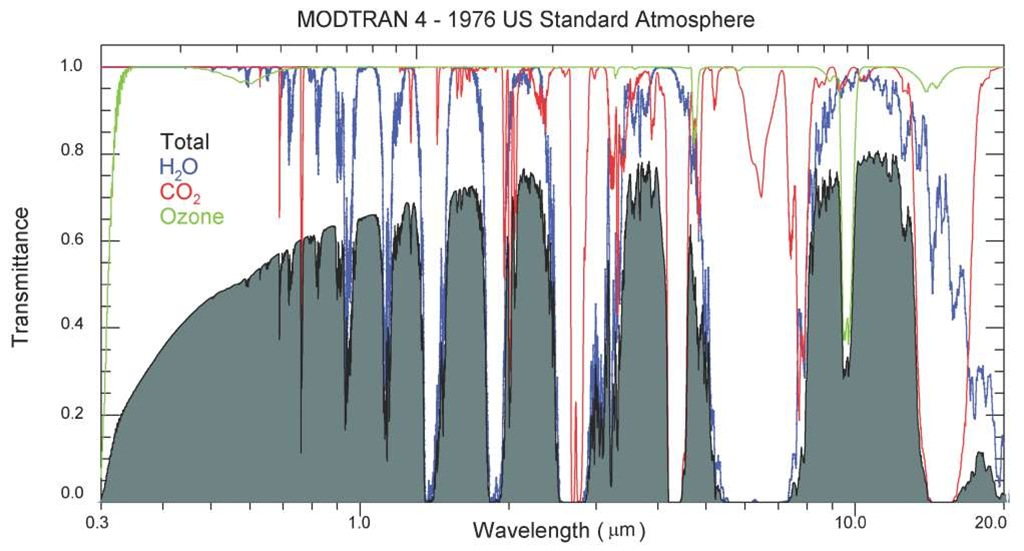
\includegraphics[width=0.9\textwidth]{figures/modtran.jpg}
\caption{\label{fig:absorption} Transmittance of atmosphere, as
reported at
\href{http://what-when-how.com/remote-sensing-from-air-and-space/atmospheric-absorption-scattering-and-turbulence-visible-imagery-remote-sensing/}{this
web site} and based on the \href{http://modtran.spectral.com/}{MODTRAN
software}. The broad band pattern is due to scattering by molecules
and aerosols.}
\end{figure}

\begin{figure}
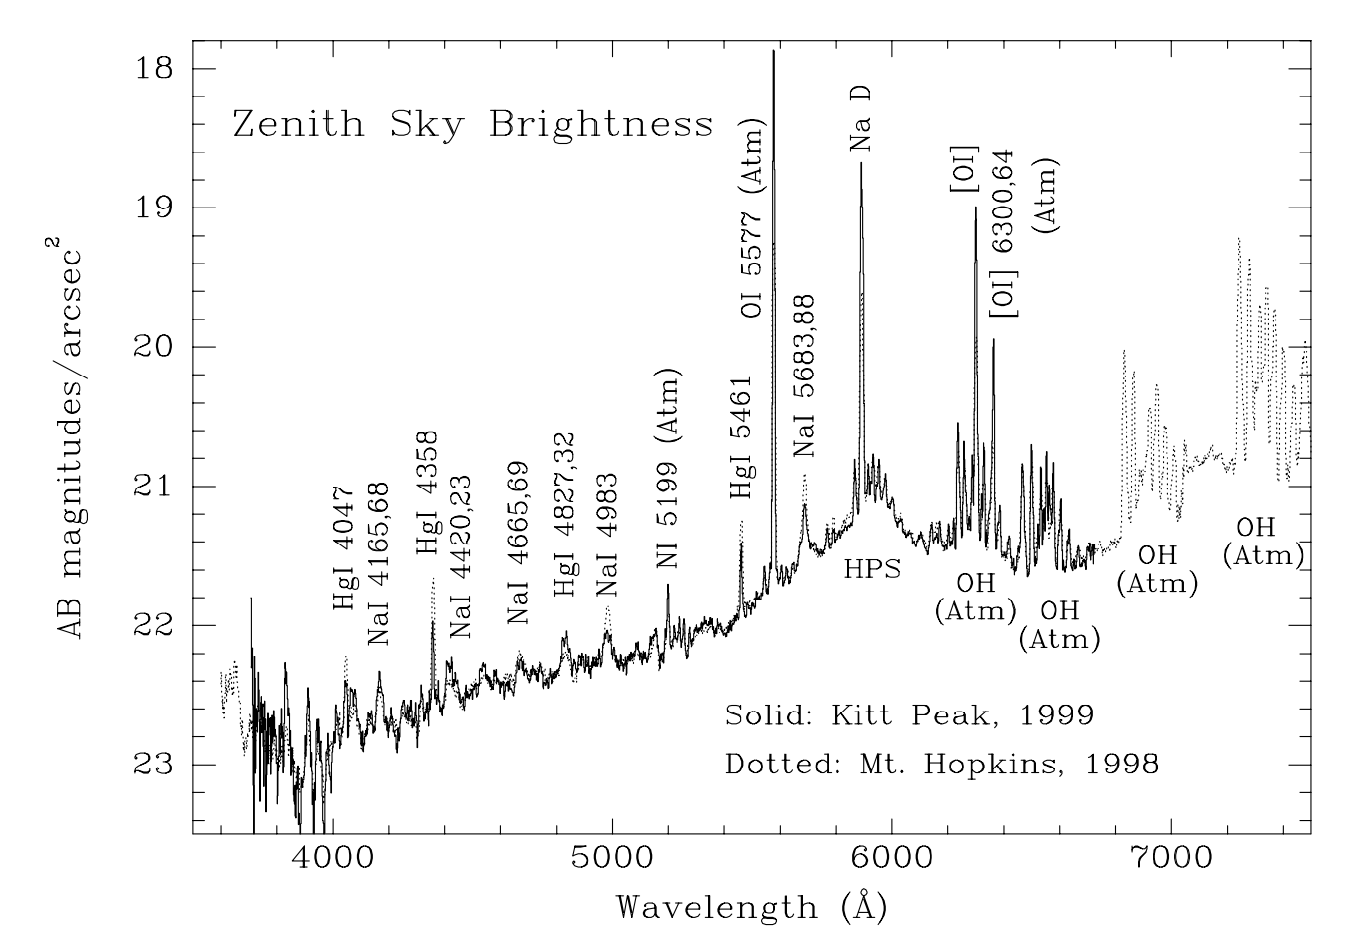
\includegraphics[width=0.9\textwidth]{figures/massey00a.png}
\caption{\label{fig:emission} Sky spectrum from \citet{massey00a}.}
\end{figure}
